	\documentclass{beamer}
	%\documentclass{abntex}

	% Pacotes
	\usepackage[utf8]{inputenc}

        %% Cores Beamer
        \setbeamercolor{item projected}{bg=darkred}
        \setbeamertemplate{enumerate items}[default]
        \setbeamertemplate{navigation symbols}{}
        \setbeamercovered{transparent}
        \setbeamercolor{block title}{fg=darkred}
        \setbeamercolor{local structure}{fg=darkred}

        %%
        \usepackage[utf8]{inputenc}              %%Formatação de acentos
        \usepackage{xcolor}                      %%Definição de cores
        \usepackage[framemethod=tikz]{mdframed} %%Estilização dos slides
        \usepackage{tcolorbox}                   %%Mudar ambientes de blocos

        % \tcbset{colback=red!5!white,
        % colframe=red!75!black,fonttitle=\bfseries} %% Borda das caixas

        \usepackage[activate={true,nocompatibility},final,tracking=true,kerning=true,spacing=true,factor=1100,stretch=10,shrink=10,expansion]{microtype}
        %% Melhorar caligrafia

        \SetTracking{encoding={*}, shape=sc}{0} %Caligrafia de small capitals (smallcaps)


        \usepackage{pifont} %Dingbats (simbolos do itemize)



	%% Configurações do Template, Imagem de Fundo[../template7.jpg], e Tema de apresentação[Madrid]
	\usebackgroundtemplate{
	  
\includegraphics[width=\paperwidth,
	  height=\paperheight]{../Imagens/fundo1.jpg}
	}
        \usetheme{Madrid}
        \usecolortheme{seahorse}

	%% Mudança de dimenções da apresentação
	\mode<presentation>


	%% Produção da Capa de Aprensentação
	\title[Relatórios]{\Huge{Produção de Relatórios, Pacote ABNTeX}}
	\author[Branquinho]{Pedro Gomes Branquinho \\
	  \text{\scriptsize{pedro.branquinho@usp.br}}}
	\date[ABNTeX]{\scriptsize{Mini-curso de \LaTeX \\ Universidade de São Paulo - DEMAR}}


	%% Início do documento
	\begin{document}

	%%Para a Capa, usaremos uma imagem diferente, com o brasão da USP, e logomarca.
	{\usebackgroundtemplate{
\includegraphics[width=\paperwidth]{../Imagens/TP.jpg}}
	  \begin{frame}
	    \titlepage
	  \end{frame}
	}

	%% Notas de versões anteriores
	% \begin{frame}
	%   \frametitle{Apesentação em \LaTeX}
	%   \tableofcontents[pausecontents]
	% \end{frame}


	%%Início da Apresentacão, o que esperar
	\begin{frame}
	  \section{Motivações}
	  \frametitle{Motivações}

	  \begin{enumerate}
	  \item<1->{Alto Nível de Produção Texual}
	  \item<3->{Auto-produção dos Índices, Indexação}
	  \item<2->{Tabelas modelo IBGE}
	  \item<4->{Fórmulas Matemáticas}
	  \item<6->{Formatação de Figuras - Imagens e Gráficos}
	  \item<5->{Referências}
	  \end{enumerate}

	\end{frame}

	\begin{frame}

	  \section{Pacote ABNTeX}
	  \frametitle{O que é, e como usar o pacote abnTeX}
	  \pause
	  \setbeamercolor{block title}{fg=white,bg=blue!75!black}
	  \begin{block}{ABN\TeX}
	    O pacote abnTeX se trata da construção de comandos de formatações
	    dentro das normas a ABNT NBR 14724:2011 e a ABNT NBR 6024:2012, as
	    quais englobarem os requisitos das demais normas ABNT de produção
	    textual. Utilizaremos largamente os \alert{``Modelos Canônicos''} da classe.
	  \end{block}
	  \pause
	 \setbeamercolor{block title}{fg=white,bg=red!75!black}
	  \begin{block}{Modelos Canônicos}
	  São documentos os quais seguem estritamente as normas ABNT. Porém,
	  não necessariamente as especificações de uma intituição. As
	  instituições brasileiras adotam particularidades, com pequenas
	  variações, em relação aos modelos canônicos.
	 \end{block}

	%   \begin{example}[Exemplos]
	%     \begin{itemize}

	%     \item O Emacs, Vim, Atom, Visual Studio, etc. são interfaces gráficas unificadas. O
	%       Emacs recebe título de IDE(Integrated Development Environment)

	%       \pause

	%     \item Jupiterweb, Moodle, Dedalus são sitemas integrados acadêmicos da
	%       USP.
	%       \pause
	%     \item O HTML + CSS são linguagens marcadoras de texto para produção web.
	%       \pause
	%     \item O \alert{\LaTeX} é uma linguagem - marcadora de texto - para produção de documentos
	%       que tenham conteúdo multimídia.
	%     \end{itemize}
	%   \end{example}
	 \end{frame}


	 \begin{frame}

	  \frametitle{Usando a classe abnTeX}
	  \pause

	  No preâmbulo do documento, carregue os pacotes presentes
	  no modelo canônico de relatórios técnicos. E, a classe do documento
	  como ``abntex2'' - as opções, 12pt, openright, etc. são parâmetros configuráveis.

	  \pause
	  \begin{center}
	    \includegraphics<-3>[width=8cm,height=7cm]{../Imagens/A2I1.png}
	  \end{center}

	\end{frame}

	\begin{frame}
	  \section{Funcionalidades}
	  \frametitle{Sumário, Indíces}

	  \begin{itemize}
	  \item Comando para produção de Sumário
	  \end{itemize}

	  %\pause

	 \begin{center}
	    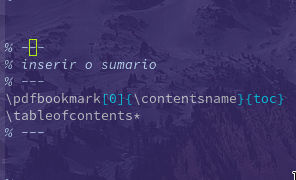
\includegraphics[scale=0.6]{../Imagens/A2I2.png}
	    %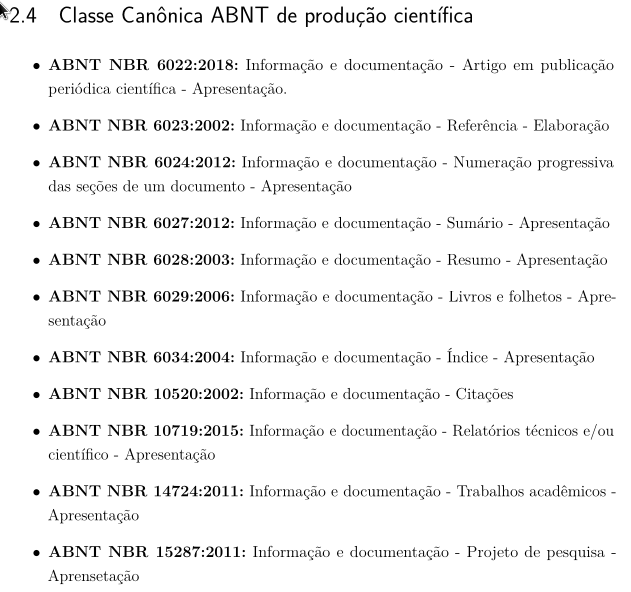
\includegraphics[width=5.5cm,height=5cm]{../Imagens/A2I22.png}
	  \end{center}
	\end{frame}




	\begin{frame}
	%  \section{Funcionalidades}
	  \frametitle{Sumário, Indíces}

	   \begin{itemize}
	  \item Auto-produção dos Índices, Indexação
	  \end{itemize}

	  %\pause

	 \begin{center}
	    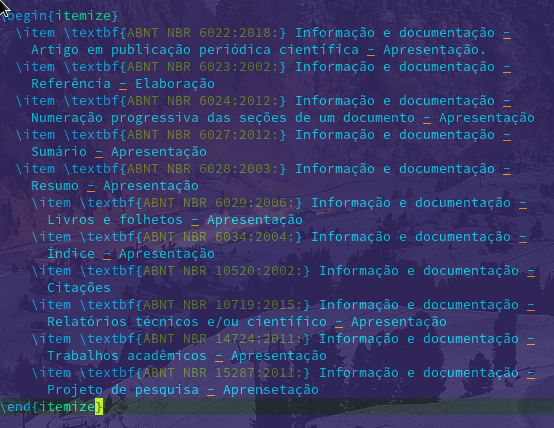
\includegraphics[width=5.5cm,height=5cm]{../Imagens/A2I21.png}
	    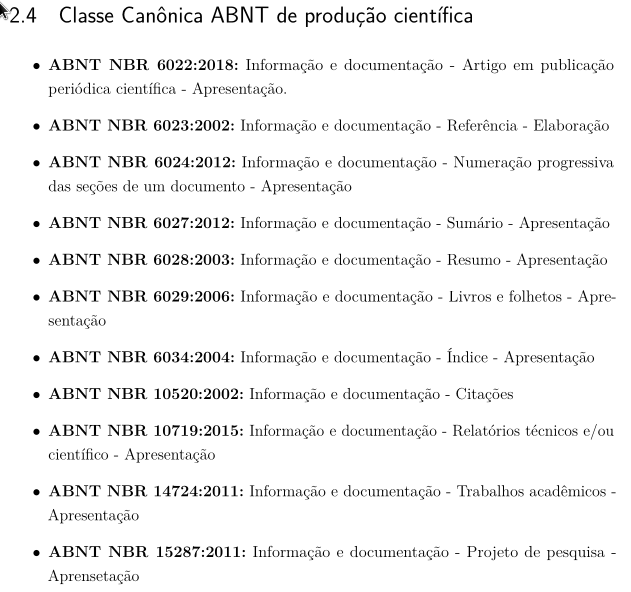
\includegraphics[width=5.5cm,height=5cm]{../Imagens/A2I22.png}
	  \end{center}
	\end{frame}


	\begin{frame}
	%  \section{Funcionalidades}
	  \frametitle{Sumário, Indíces}

	   \begin{itemize}
	  \item Auto-produção dos Índices, Indexação
	  \end{itemize}

	 \begin{center}
	    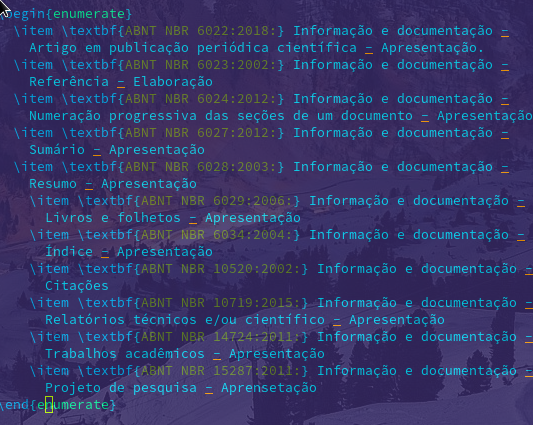
\includegraphics[width=5.5cm,height=5cm]{../Imagens/A2I31.png}
	    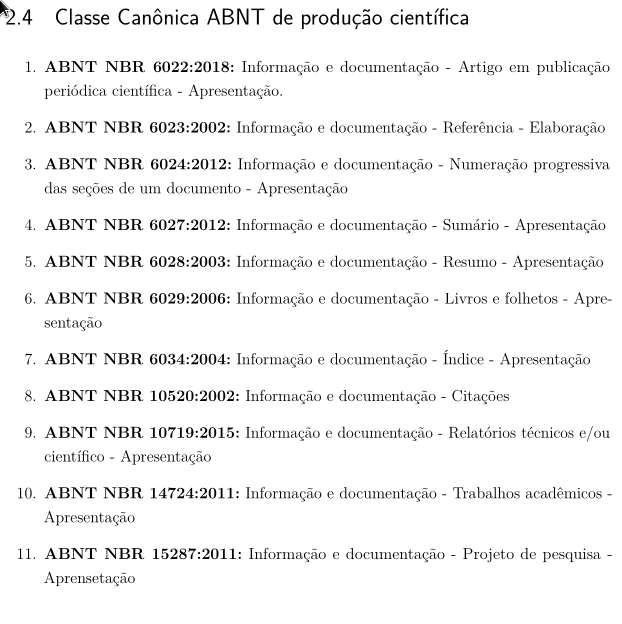
\includegraphics[width=5.5cm,height=5cm]{../Imagens/A2I32.png}
	  \end{center}
	\end{frame}


	%   \pause

	%    \begin{center}
	%   %  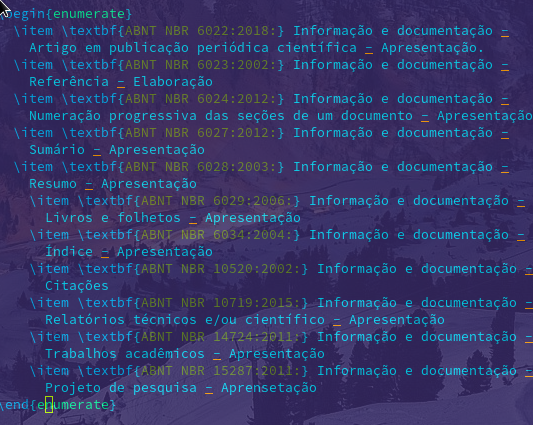
\includegraphics[width=4cm,height=3.5cm]{../Imagens/A2I31.png}
	%    % 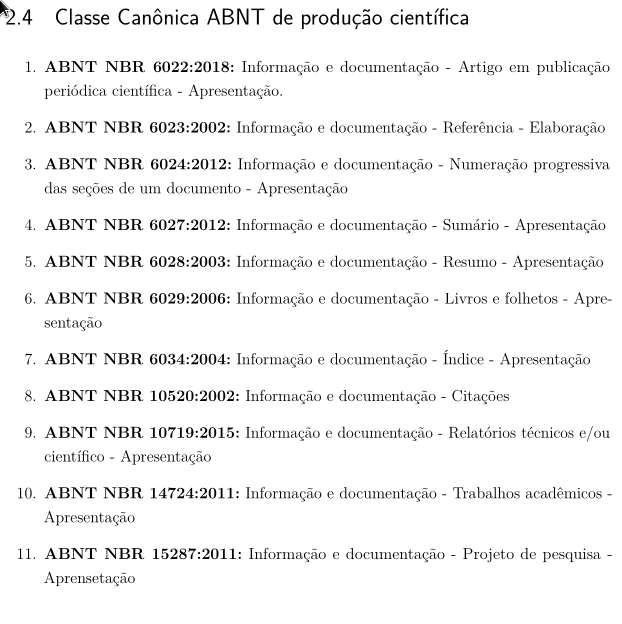
\includegraphics[width=4cm,height=3.5cm]{../Imagens/A2I32.png}
	%   \end{center}

	\begin{frame}
	%  \section{Funcionalidades}
	  \frametitle{Sumário}

	   \begin{itemize}
	   \item Formatação textual lógica-sequencial
	  \end{itemize}

	 \begin{center}
	    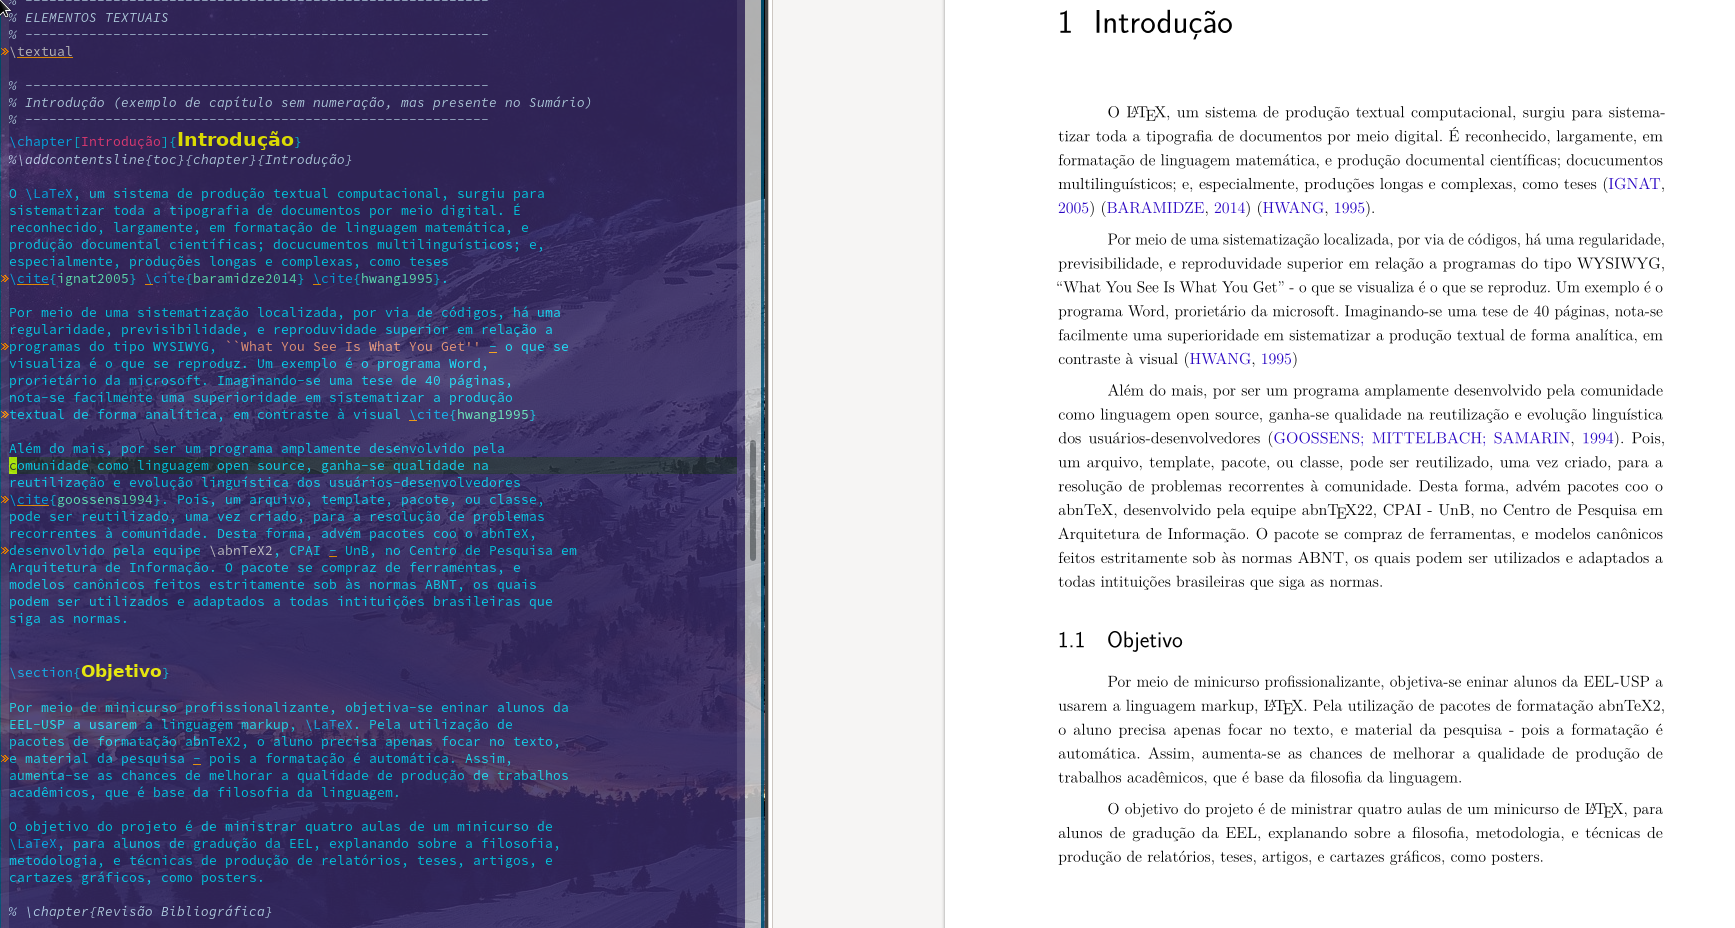
\includegraphics[width=12cm,height=7cm]{../Imagens/A2I41.png}
	%    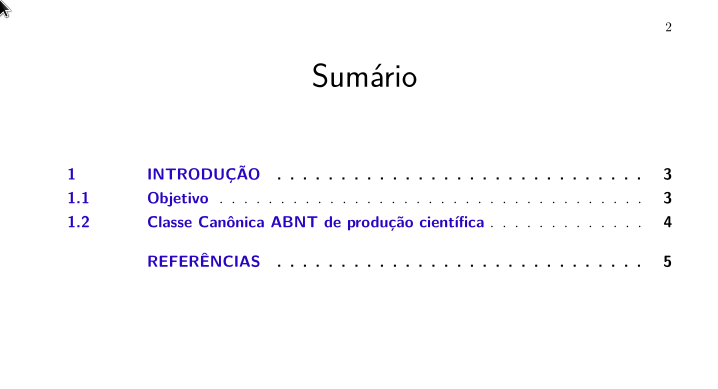
\includegraphics[width=5.5cm,height=5cm]{../Imagens/A2I42.png}
	  \end{center}

	\end{frame}

	\begin{frame}
	%  \section{Funcionalidades}
	  \frametitle{Sumário}

	   \begin{itemize}
	  \item Auto-produção dos Sumários
	  \end{itemize}

	 \begin{center}
	%  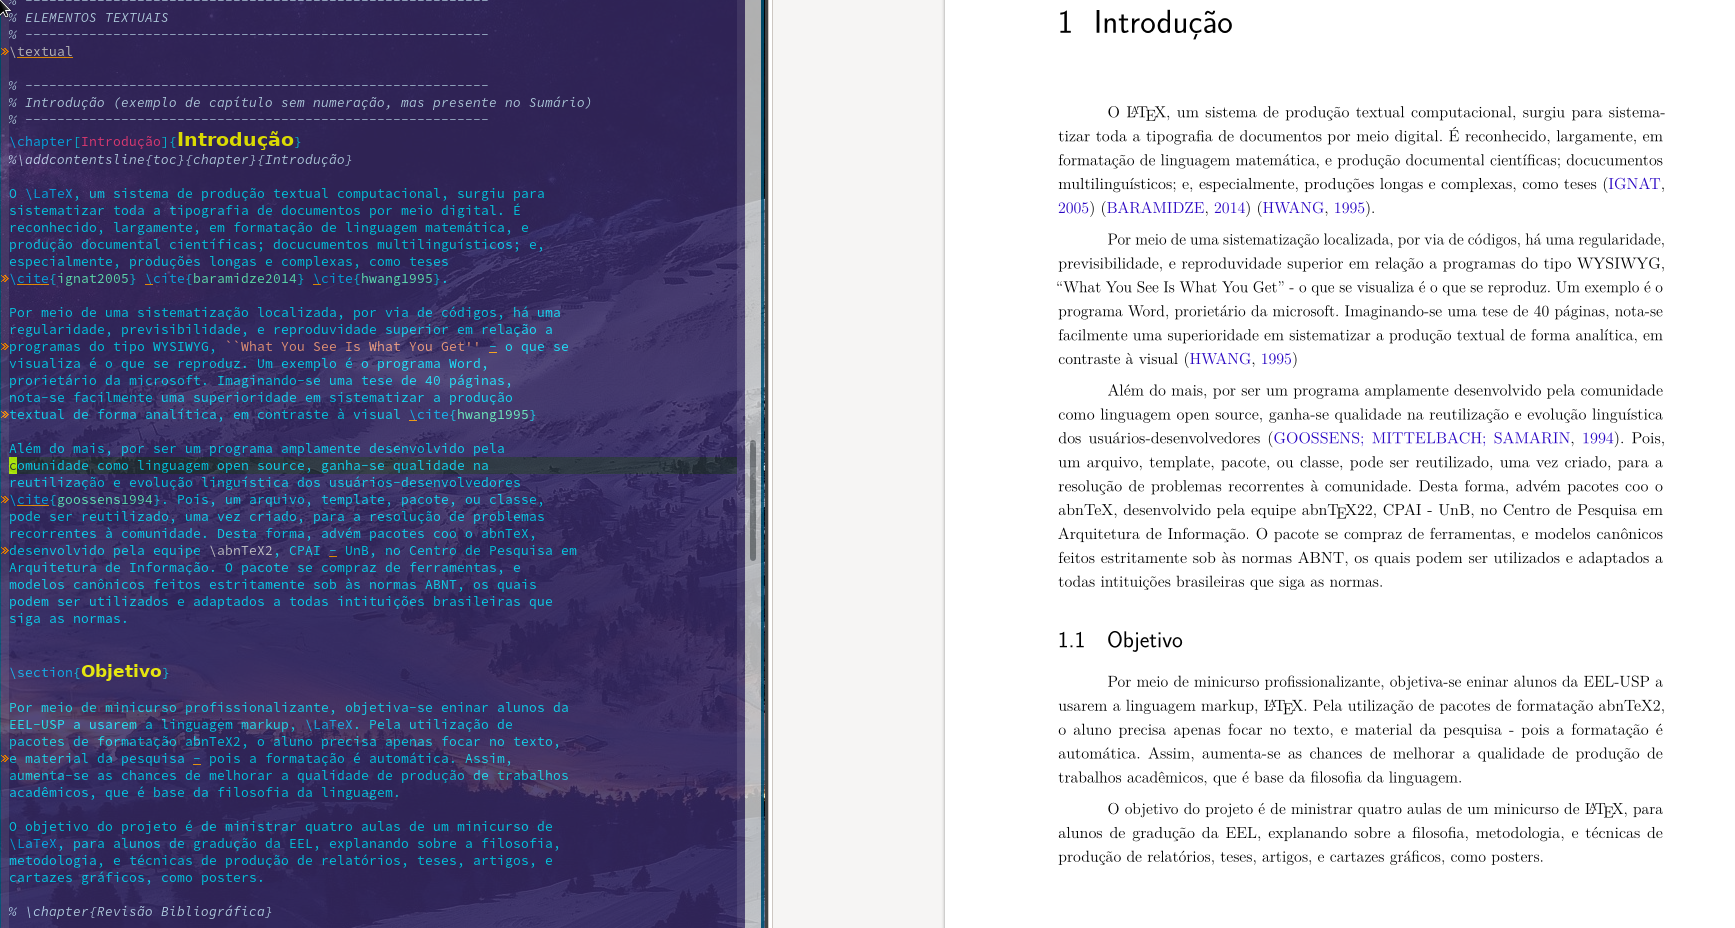
\includegraphics[width=5.5cm,height=5cm]{../Imagens/A2I41.png}
	   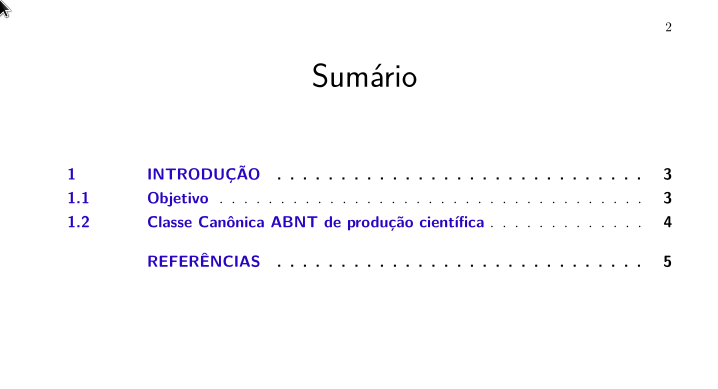
\includegraphics[scale=0.4]{../Imagens/A2I42.png}
	  \end{center}

	\end{frame}

	% \begin{frame}
	% %  \section{Funcionalidades}
	%   \frametitle{Sumário}

	%    \begin{itemize}
	%   \item Auto-produção dos Sumários
	%   \end{itemize}

	%  \begin{center}
	% %  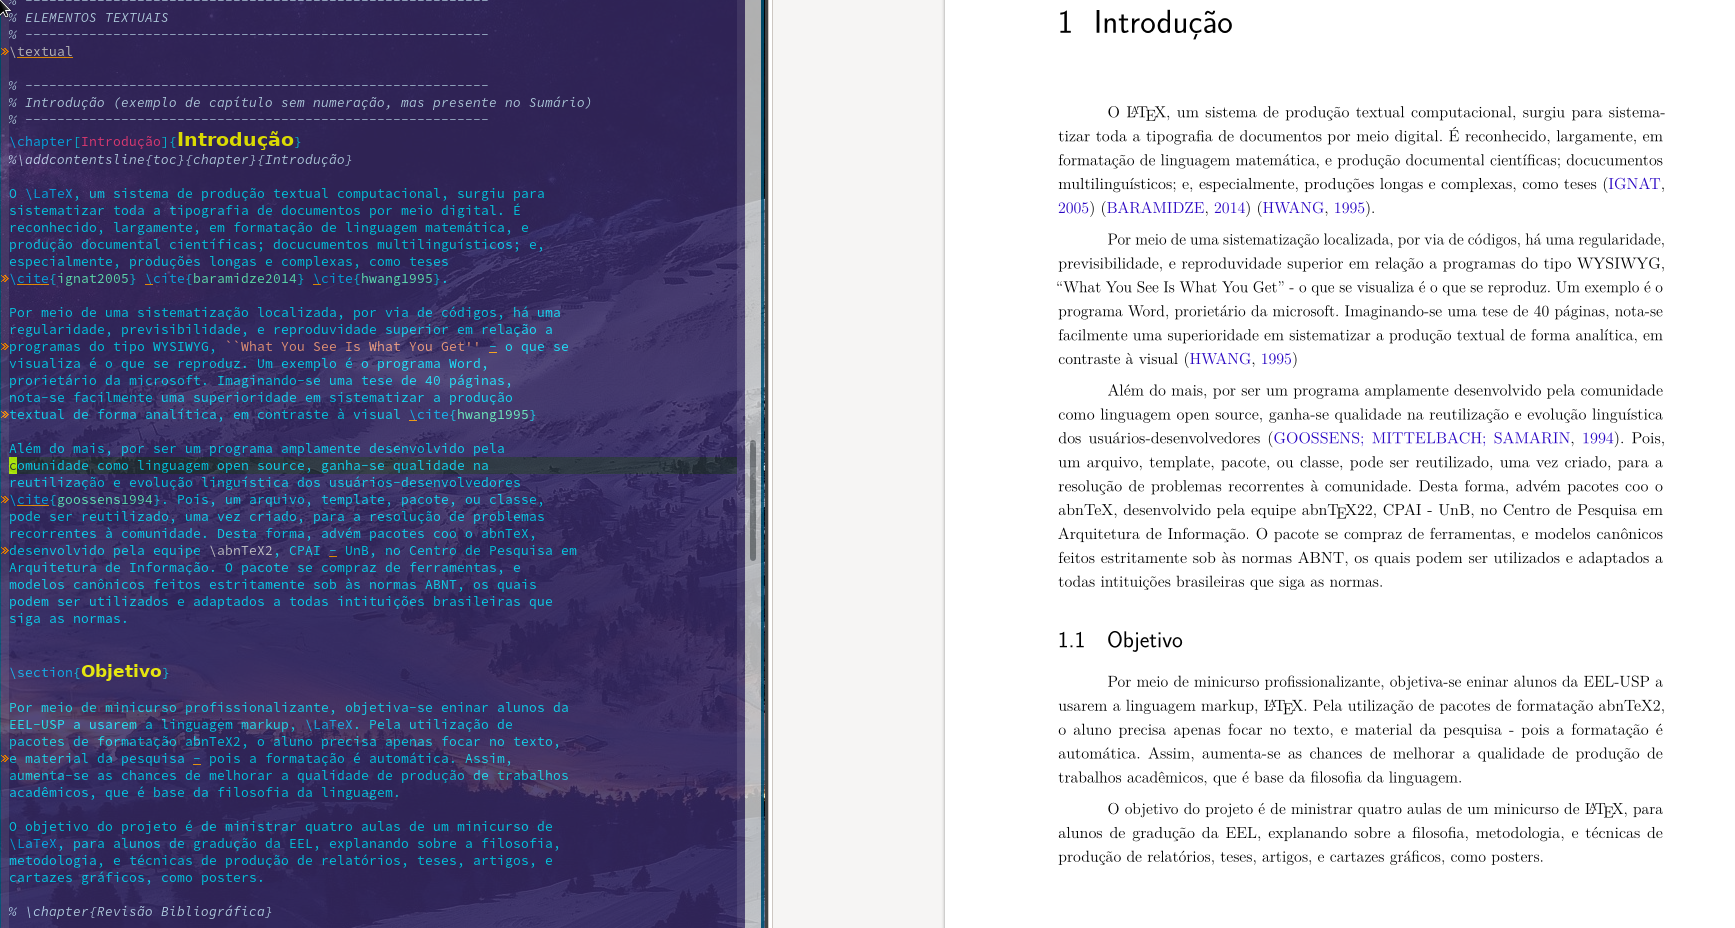
\includegraphics[width=5.5cm,height=5cm]{../Imagens/A2I41.png}
	%    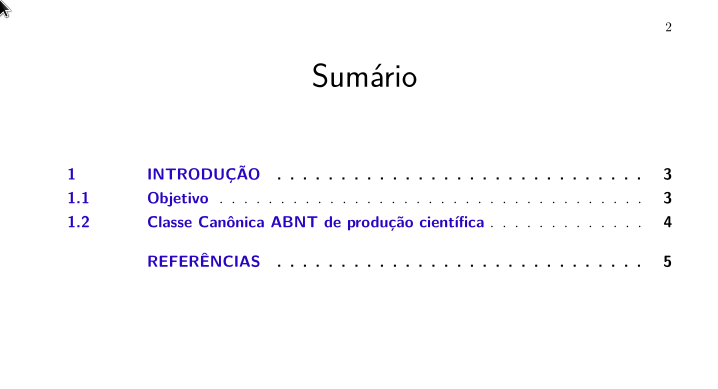
\includegraphics[width=7cm,height=5cm]{../Imagens/A2I42.png}
	%   \end{center}

	% \end{frame}


	\begin{frame}
	%  \section{Funcionalidades}
	  \frametitle{Contra-exemplo}

	   \begin{itemize}
	  \item Eventual adição de itens ao documento
	  \end{itemize}

	 \begin{center}
	   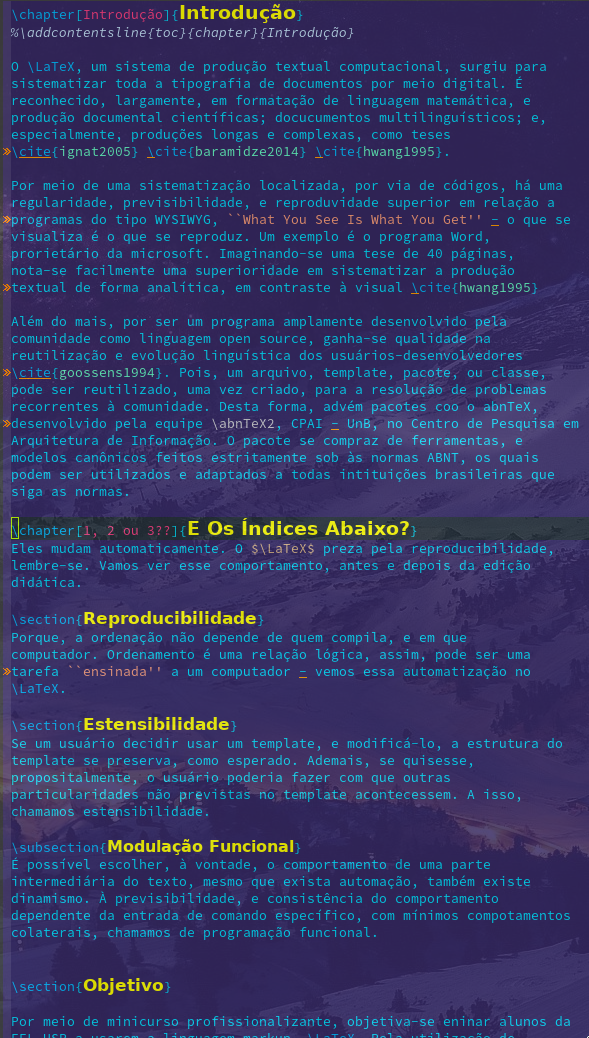
\includegraphics[scale=0.185]{../Imagens/A2I51.png}
	  \end{center}

	\end{frame}


	\begin{frame}
	%  \section{Funcionalidades}
	  \frametitle{Contra-exemplo}

	   \begin{itemize}
	  \item Comportamento esperado, índice-textual:
	  \end{itemize}

	 \begin{center}
	  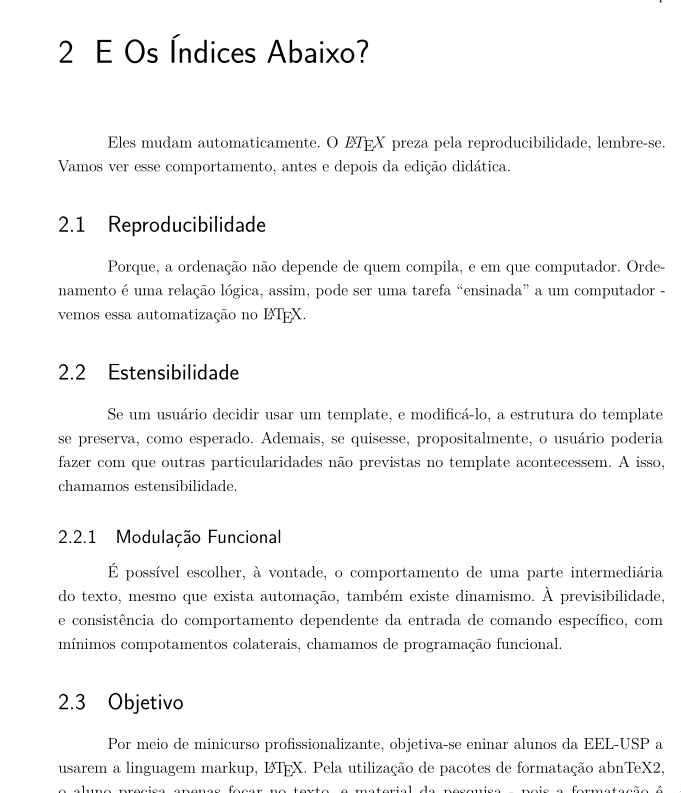
\includegraphics[scale=0.25]{../Imagens/A2I53.png}
	  \end{center}

	\end{frame}


	\begin{frame}
	%  \section{Funcionalidades}
	  \frametitle{Contra-exemplo}

	   \begin{itemize}
	  \item Comportamento esperado, sumário:
	  \end{itemize}

	 \begin{center}
	  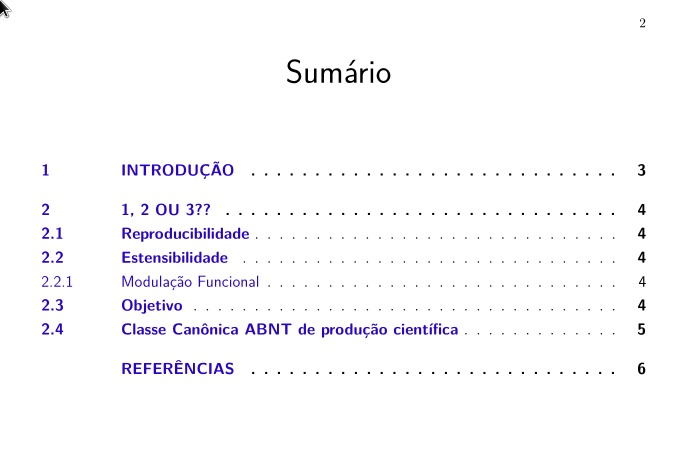
\includegraphics[scale=0.3]{../Imagens/A2I52.png}
	  \end{center}

	\end{frame}
	% \begin{frame}
	% \item<4-> Formatação de Figuras - Imagens e Gráficos
	% \end{frame}

	\begin{frame}
	  \section{Tabelas - Modelo IBGE}
	  \frametitle{Tabelas - Modelo IBGE}

	   \begin{itemize}
	  \item Ambiente Tabela || || ||  || Resultado
	  \end{itemize}

	 \begin{center}
	   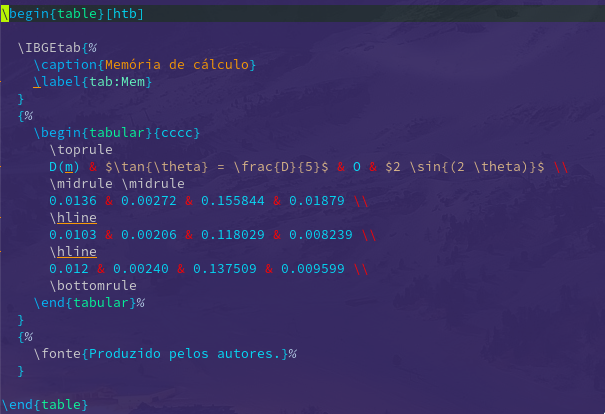
\includegraphics[scale=0.28]{../Imagens/A2I61.png}
	   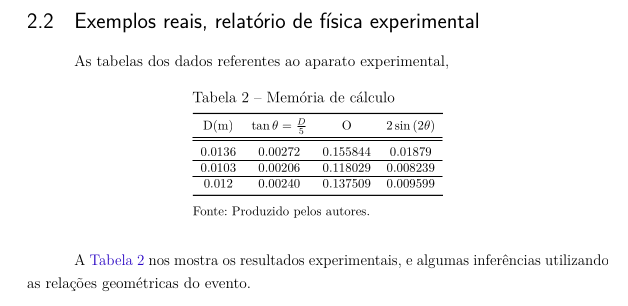
\includegraphics[scale=0.24]{../Imagens/A2I62.png}
	\end{center}

	\pause

	Nota: existe exemplos dessas formatações nos arquivos do
	repositório. Basta reutilizá-los para tabelas, imagens, e fórmulas.

	\end{frame}

	\begin{frame}
	  \section{Fórmulas Matemáticas}
	  \frametitle{Fórmulas Matemáticas}

	   \begin{itemize}
	  \item Ambiente de Fórmula || || || Resultado
	  \end{itemize}
	    % \~\~ \\
	  %   \~\~ \\
	 \begin{center}
	   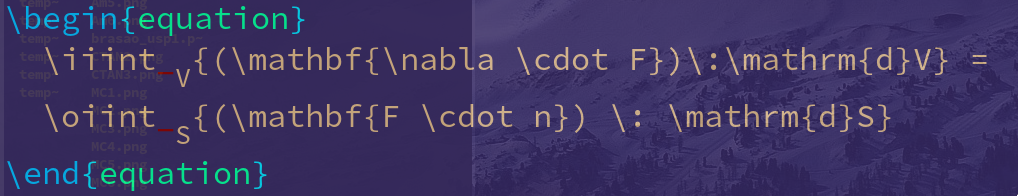
\includegraphics[scale=0.30]{../Imagens/A2I71.png}
	  % \~\~ \\
	 %  \~\~ \\
	   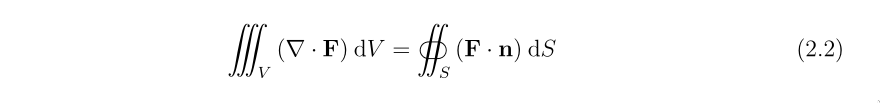
\includegraphics[scale=0.40]{../Imagens/A2I72.png}
	\end{center}
	\end{frame}



	% \begin{frame}
	%   \section{Formatação de  Imagens}
	%   \frametitle{Ambiente de Imagens}
	%  % \\~~
	%   Esse é o código usado para formatar uma imagem da apresentação:
	%    \begin{center}
	%    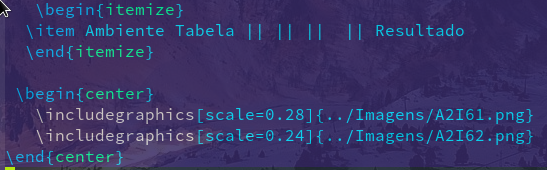
\includegraphics[scale=0.30]{../Imagens/A2I91.png}
	%  \end{center}
	% % \\~~
	%  Resultado:
	%  \begin{center}
	%    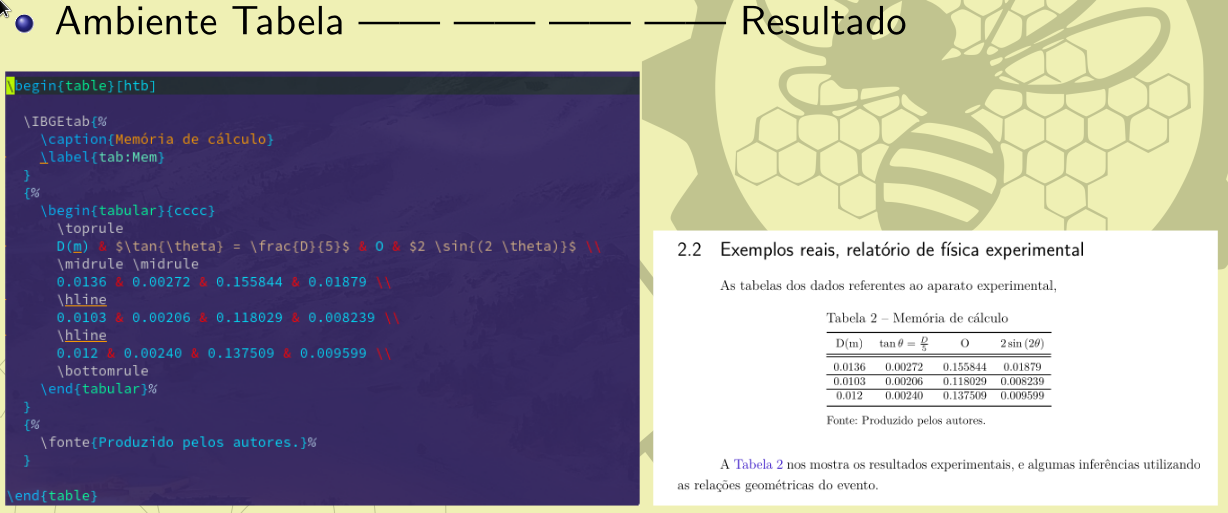
\includegraphics[scale=0.23]{../Imagens/A2I92.png}
	% \end{center}
	% \end{frame}


	\begin{frame}
	  \section{Formatação de  Imagens}
	  \frametitle{Ambiente de Imagens}
	  \\~~
	  Esse é o código usado para formatar uma imagem da apresentação:
	   \begin{center}
	   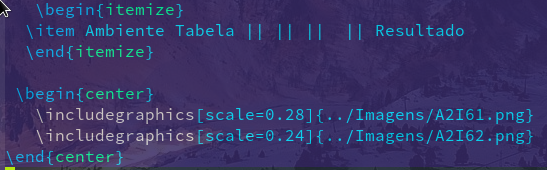
\includegraphics[scale=0.30]{../Imagens/A2I91.png}
	 \end{center}
	 \\~~
	 Resultado:
	 \begin{center}
	   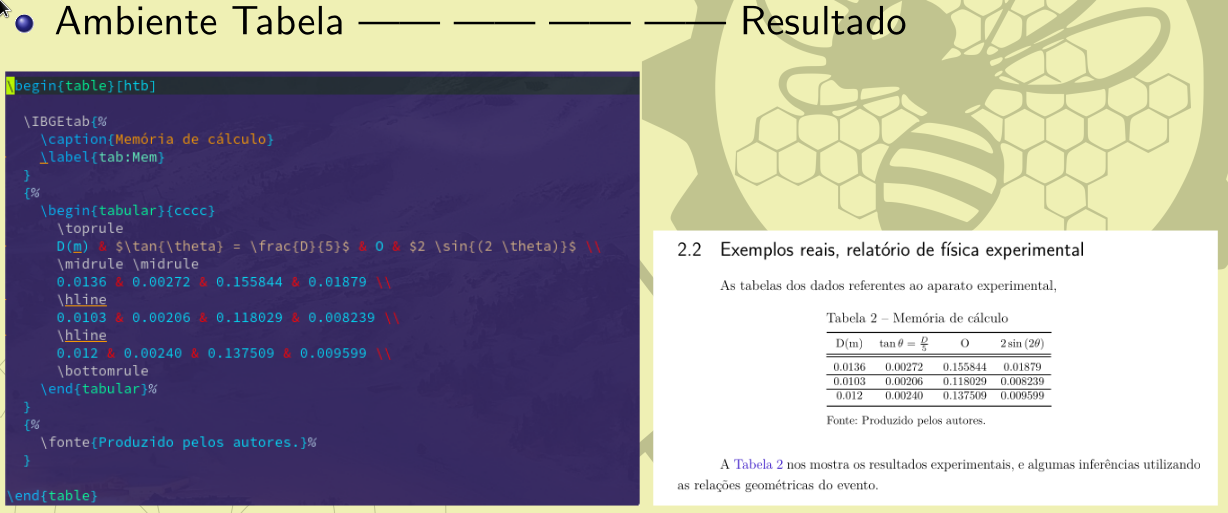
\includegraphics[scale=0.23]{../Imagens/A2I92.png}
	\end{center}
	\end{frame}

	\begin{frame}
	 \section{Formatação de Referências}
	  \frametitle{Arquivo ``.bib''}

	  \begin{itemize}
	  \item O arquivo .bib é um banco de dados estruturado, de onde chama-se
	  dados para construir citações e refências bibliográficas.
	\end{itemize}

	\\~~

	Exemplo do conteúdo do arquivo,
	\begin{center}
	  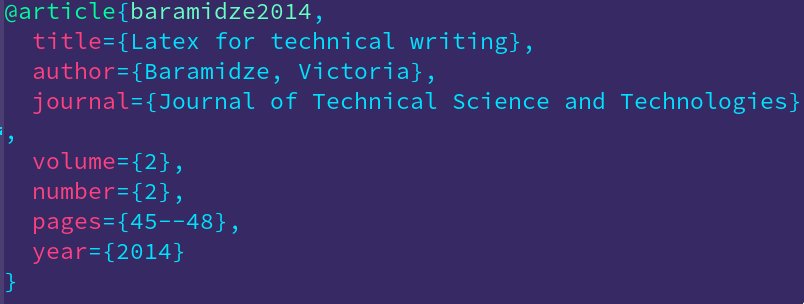
\includegraphics[scale=0.40]{../Imagens/A2I101.png}
	\end{center}
	\end{frame}

	\begin{frame}
	  \frametitle{Referência tipo BibTeX}

	  \begin{itemize}
	  \item O nome dado a essa estrutura dos dados é do tipo BibTex. E, é
	    possível acessá-las prontas na Internet.
	\end{itemize}

	\\~~

	Pelo Google Scholar,
	\begin{center}
	  
\includegraphics[scale=0.20]{../Imagens/A2I102.png}
	\end{center}
	\\~~
	(Clicar no símbolo de aspas: '' - canto inferior esquerdo do artigo)


	\end{frame}

	\begin{frame}

	  \frametitle{Citação formato BibTeX}

	  \begin{itemize}
	  \item É possível escolher formatações de diversos bancos de
	    dados. Utilizaremos a opção BibTex.
	\end{itemize}

	\\~~

	\begin{center}
	  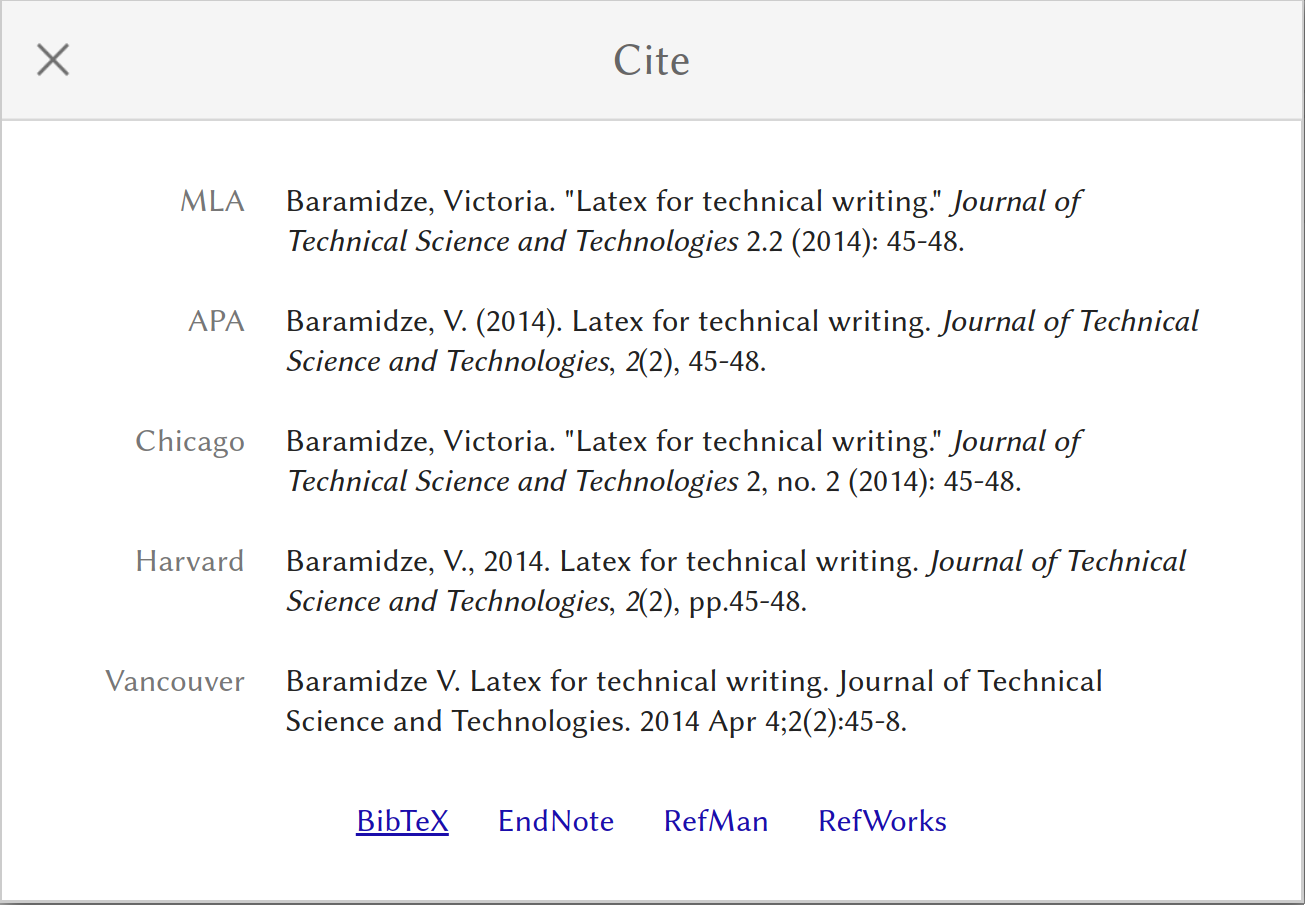
\includegraphics[scale=0.15]{../Imagens/A2I103.png}
	  (Clicar em BibTex, canto inferior esquerdo)
	\end{center}


	\end{frame}

	\begin{frame}

	  \frametitle{Citação formato BibTeX}

	  \begin{itemize}
	  \item Copiar e colar a informação para o seu arquivo de extenção .bib
	\end{itemize}

	\\~~

	\begin{center}
	  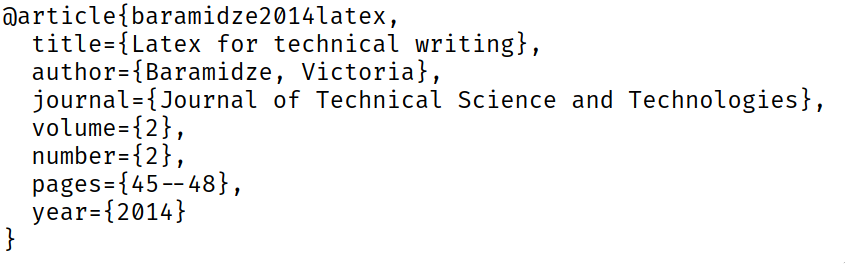
\includegraphics[scale=0.30]{../Imagens/A2I104.png}
	\end{center}


	\end{frame}


	\begin{frame}[fragile]

	  \frametitle{Citações - Documento Principal}

	  \begin{itemize}
	  \item Comando \verb_\cite{AutorAno}_ e seu resultado, na prática.
	\end{itemize}

	\\~~

	\begin{center}
	  Comando: \\
	  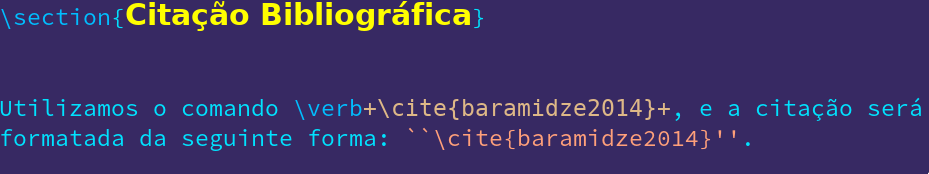
\includegraphics[scale=0.30]{../Imagens/A2I111.png}

	  \\~~

	  Resultado: \\
	  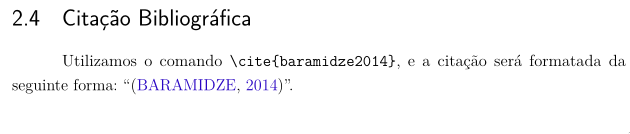
\includegraphics[scale=0.40]{../Imagens/A2I112.png}
	\end{center}

	\end{frame}

	\begin{frame}[fragile]
	  \frametitle{Referências Bibliográficas - Documento Principal}
	  \begin{itemize}
	  \item Comando \verb_\bibliography{Diretório/Nome-Arquivo-Bib}_ e seu resultado, na prática.
	  \end{itemize}
	  \\~~
	\begin{center}
	  Comando, ao fim do documento:
	  \\~~
	  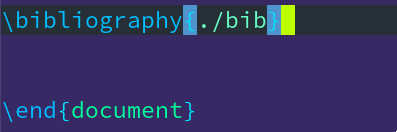
\includegraphics[scale=0.60]{../Imagens/A2I122.png}
	\end{center}

	\end{frame}

	\begin{frame}[fragile]
	  \frametitle{Referências Bibliográficas - Documento Principal}
	  \begin{itemize}
	  \item Comando \verb_\bibliography{Diretório/Nome-Arquivo-Bib}_ e seu resultado, na prática.
	  \end{itemize}
	\begin{center}
	  Resultado: \\
          \vspace{0.4cm}

	  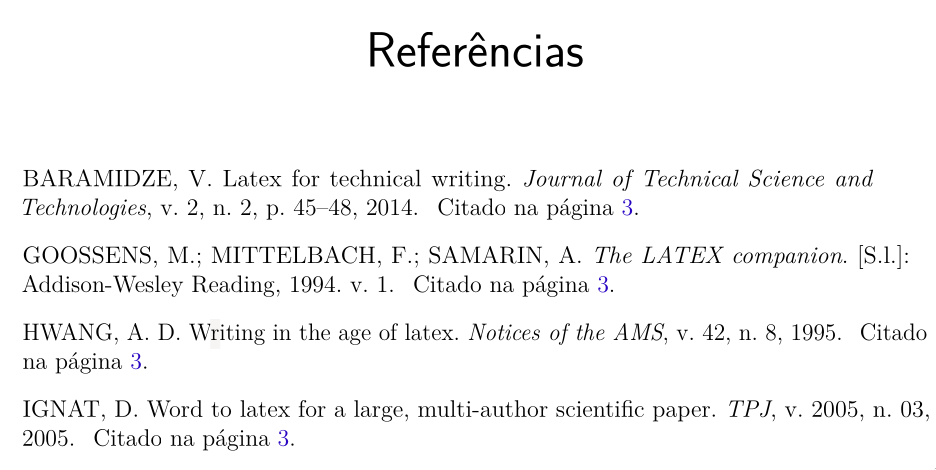
\includegraphics[scale=0.30]{../Imagens/A2I121.png}
	\end{center}
	\end{frame}

	% \begin{frame}[fragile]

	%   \frametitle{Referências Fórmulas e Tabelas}

	%   \begin{itemize}
	%   \item Comandos \verb_\label{meuLabel}_  e \verb_\autoref{meuLabel}_
	%   \end{itemize}

	%   \begin{center}
	%     Resultado: \\
	%     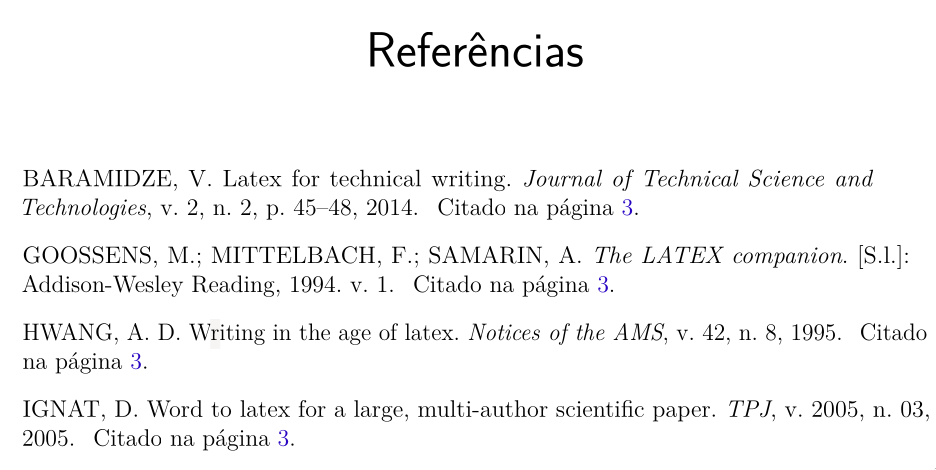
\includegraphics[scale=0.30]{../Imagens/A2I121.png}
	%   \end{center}

	% \end{frame}



	\end{document}

	%%% Local Variables:
	%%% mode: latex
	%%% TeX-master: t
	%%% End:

	%%% Local Variables:
	%%% mode: latex
	%%% TeX-master: t
	%%% End:
